\documentclass[border=10pt]{standalone}
\usepackage{tikz}
\usetikzlibrary{matrix}

\tikzset{
    header/.style={
        fill=blue!70!black,
        text=white,
        align=center,
        font=\bfseries,
    },
    firstcol/.style={
        fill=blue!10,
        align=left,
        font=\bfseries,
    },
    cell/.style={
        fill=white,
        align=right,
        font=\normalfont,
    },
}

\begin{document}
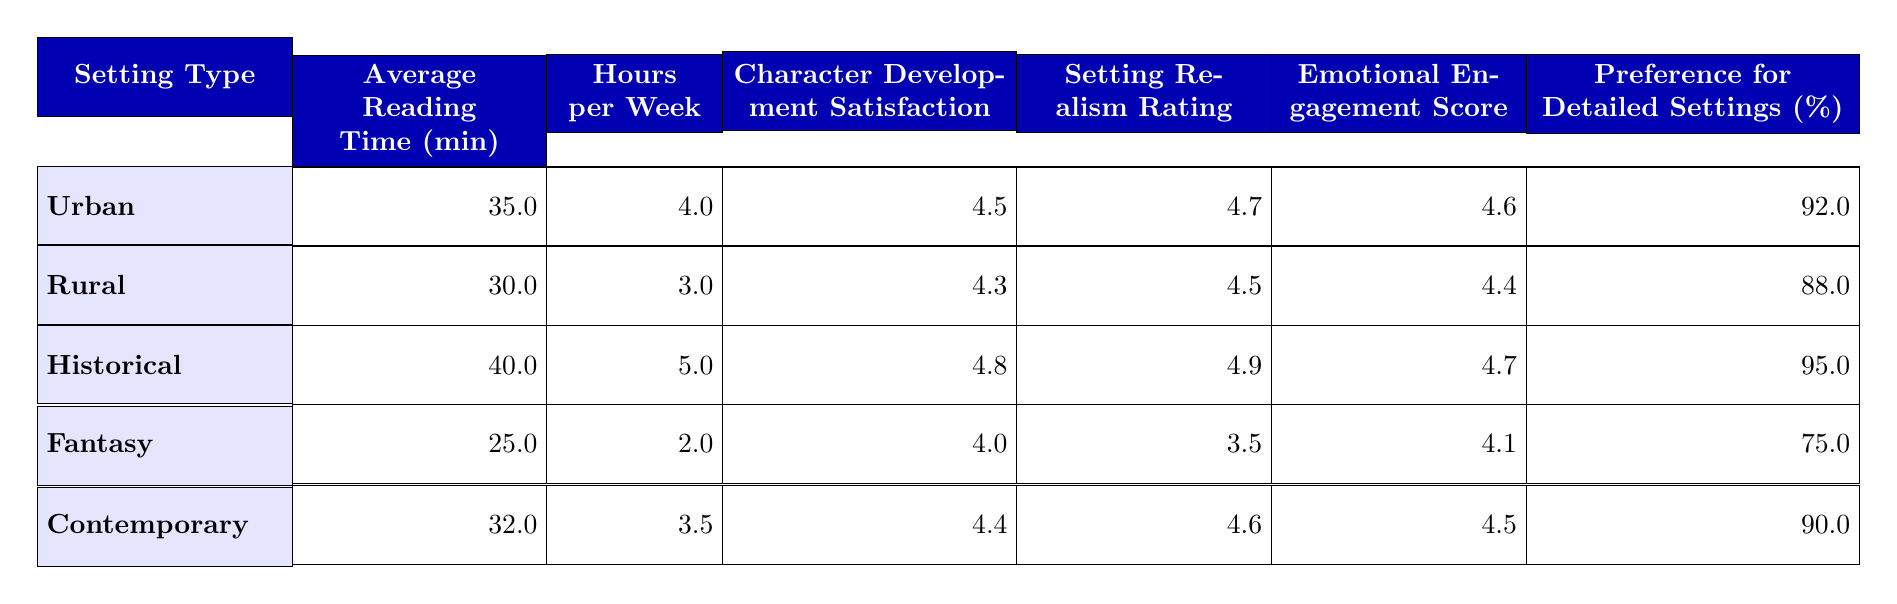
\begin{tikzpicture}
\matrix (m) [matrix of nodes, 
    nodes in empty cells,
    nodes={cell, draw=black, minimum height=1cm, text width=2.5cm},
    column 1/.style={nodes={text width=3cm}},
    column 2/.style={nodes={text width=3cm}},
    column 3/.style={nodes={text width=2cm}},
    column 4/.style={nodes={text width=3.5cm}},
    column 5/.style={nodes={text width=3cm}},
    column 6/.style={nodes={text width=3cm}},
    column 7/.style={nodes={text width=4cm}},
    column sep=-\pgflinewidth,
    row sep=-\pgflinewidth
] {
    |[header]| Setting Type & |[header]| Average Reading Time (min) & |[header]| Hours per Week & |[header]| Character Development Satisfaction & |[header]| Setting Realism Rating & |[header]| Emotional Engagement Score & |[header]| Preference for Detailed Settings (\%) \\
    |[firstcol]| Urban & 35.0 & 4.0 & 4.5 & 4.7 & 4.6 & 92.0 \\
    |[firstcol]| Rural & 30.0 & 3.0 & 4.3 & 4.5 & 4.4 & 88.0 \\
    |[firstcol]| Historical & 40.0 & 5.0 & 4.8 & 4.9 & 4.7 & 95.0 \\
    |[firstcol]| Fantasy & 25.0 & 2.0 & 4.0 & 3.5 & 4.1 & 75.0 \\
    |[firstcol]| Contemporary & 32.0 & 3.5 & 4.4 & 4.6 & 4.5 & 90.0 \\
};
\end{tikzpicture}
\end{document}